\chapter{Risk as Controllable Variables}

This chapter is based on a short School of Hard Knocks entrepreneurship interview, curated by LazyingArt LLC with Video2Book. The spoken exchange asks a practical question: what is the most important part of taking risks to become successful, including risks outside finance? The answer does not glorify risk for its own sake. It turns risk into a sorting problem: first ask what can be mitigated, fixed, or controlled; then ask whether the remaining uncertainty fits the entrepreneur's tolerance.

\section{The Question: What Makes Risk Worth Taking?}

The question comes in two parts. First, what matters most about taking risks in order to become successful? Second, are there risks outside finance that had to be taken along the way? That framing is important because the answer is not merely about money. It is about judgment under uncertainty.

The speaker begins with a broad claim: there are many ways to think about risk. Then he immediately narrows the useful version of the question. In the companies he works with, and in the places he worked before, the operative question is not simply whether a situation is risky. The operative question is whether the risk can be mitigated or fixed.

\begin{definition}
A \emph{risk variable} is a material uncertainty that can affect the outcome of a decision. A variable is \emph{controllable} if the entrepreneur can meaningfully influence, mitigate, or repair it. A variable is \emph{uncontrollable} if it lies outside the entrepreneur's practical reach.
\end{definition}

The chapter will use a small amount of notation, but only as a disciplined shorthand for the interview's concrete examples. Let
\begin{equation}
n=\hbox{number of material risk variables}, \qquad
c=\hbox{number that can be controlled or mitigated}.
\end{equation}
Then the descriptive controllability ratio is
\begin{equation}
\rho=\frac{c}{n}.
\end{equation}
This is not a probability of success. It is a compact way to keep track of the speaker's distinction between risks one can work on and risks one merely suffers.

\section{Risk as Control, Not Drama}

A common entrepreneurial mistake is to treat risk as if its value comes from boldness alone. The speaker cuts against that idea. If a risk is way outside one's control, then it is outside one's control. That sounds almost too plain, but it is the center of the lesson.

The test is not whether the decision feels ambitious. The test is whether the entrepreneur can act on enough of the moving parts. A risk that can be mitigated or fixed belongs to the world of operating judgment. A risk with too many uncontrollable variables belongs closer to gambling.

\subsection{Question \& Answer}

\paragraph{Question.}
When is a risk worth taking?

\paragraph{Answer.}
A risk becomes worth considering when enough of the important variables are controllable, mitigable, or fixable. If the important variables are mostly outside control, the decision is not disciplined risk; it is a flyer. Even when enough variables are controllable, the decision still depends on the entrepreneur's risk tolerance.

We can write the local rule as a cautious mnemonic:
\begin{equation}
\hbox{disciplined risk}
\quad \approx \quad
\hbox{controllable variables}
+
\hbox{tolerance for the remainder}.
\end{equation}
The symbol \(\approx\) matters. The interview does not give a formula for success. It gives a way to discipline the first question.

\section{Counting the Variables}

The speaker's numerical examples make the idea concrete. Suppose there are six risky variables and only two can be controlled. In our notation,
\begin{equation}
n=6,\qquad c=2,\qquad \rho=\frac{2}{6}=\frac{1}{3}.
\end{equation}
The speaker's judgment is that this is not a good idea. We should not take a flyer and say, in effect, that six variables are loose but only two are under our influence.

Now change the structure. Suppose there are three risky variables and two can be controlled:
\begin{equation}
n=3,\qquad c=2,\qquad \rho=\frac{2}{3}.
\end{equation}
The spoken judgment changes with the structure. In that case, the entrepreneur generally has a better shot. The decision is still risky, but the risk is no longer shapeless. Two of the three important variables can be worked on.

\subsection{Worked Example: The Same Two Variables in Different Worlds}

The difference between the two cases is not the number \(c=2\) by itself. In both examples the entrepreneur can control two variables. The difference is the denominator: the number of material uncertainties that matter.

\begin{align}
\rho_{\mathrm{loose}} &= \frac{2}{6}=\frac{1}{3},\\
\rho_{\mathrm{tighter}} &= \frac{2}{3}.
\end{align}

The comparison is
\begin{equation}
\rho_{\mathrm{tighter}} > \rho_{\mathrm{loose}}.
\end{equation}
That inequality is the whole mathematical payload of the example. It does not prove success, but it explains why the second situation is more attractive: the entrepreneur controls a larger share of the variables that matter.

\begin{table}
\centering
\begin{tabular}{p{0.28\linewidth} p{0.25\linewidth} p{0.34\linewidth}}
Risk situation & Control position & Speaker's implied judgment \\
Six risky variables & Control two & Too many loose variables; do not take a flyer \\
Three risky variables & Control two & Better shot; enough may be controllable to proceed \\
\end{tabular}
\caption{A compact reconstruction of the interview's variable-counting heuristic.}
\end{table}

\section{A Decision Diagram for Mitigable Risk}

Because no validated board screenshot remains for this lecture, the following diagram is a conceptual reconstruction from the transcript rather than visual evidence from the video. It is deliberately narrow: the point is to preserve the sequence of thought, not to build a large risk model.

\begin{figure}
\centering
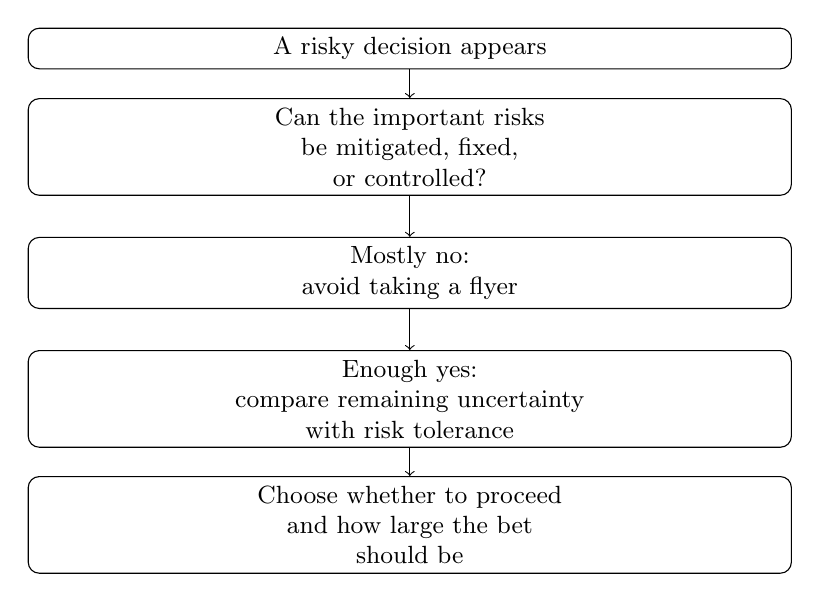
\begin{tikzpicture}[x=1cm,y=1cm,every node/.style={font=\small}]
\node[draw,rounded corners,align=center,text width=.78\linewidth] (a) at (0,0) {A risky decision appears};
\node[draw,rounded corners,align=center,text width=.78\linewidth] (b) at (0,-1.25) {Can the important risks\\ be mitigated, fixed,\\ or controlled?};
\node[draw,rounded corners,align=center,text width=.78\linewidth] (c) at (0,-2.85) {Mostly no:\\ avoid taking a flyer};
\node[draw,rounded corners,align=center,text width=.78\linewidth] (d) at (0,-4.45) {Enough yes:\\ compare remaining uncertainty\\ with risk tolerance};
\node[draw,rounded corners,align=center,text width=.78\linewidth] (e) at (0,-6.05) {Choose whether to proceed\\ and how large the bet\\ should be};
\draw[->] (a) -- (b);
\draw[->] (b) -- (c);
\draw[->] (c) -- (d);
\draw[->] (d) -- (e);
\end{tikzpicture}
\caption{Transcript-derived decision flow for the speaker's risk heuristic.}
\end{figure}

The diagram should be read vertically. The first cut is controllability. The second cut is personal tolerance. The final choice is not merely yes or no; it also concerns the size of the bet.

\section{Risk Tolerance and Bet Size}

After the variable examples, the speaker pivots to risk tolerance. This is the human side of the model. Two entrepreneurs can face the same \(\rho\) and make different decisions because they cannot absorb or accept the same remaining uncertainty.

Let \(T\) denote a person's tolerance for unresolved risk. We should not pretend that \(T\) is measured precisely here. It is a reminder that controllability is necessary but not sufficient. In a compact form:
\begin{equation}
\hbox{decision quality depends on }(\rho,T),
\end{equation}
where \(\rho\) describes the structure of the situation and \(T\) describes the person's willingness to carry what remains.

The speaker then moves from tolerance to bet size. If the risk is acceptable, one still has to decide how much to put behind it. A small bet and a large bet can face the same underlying opportunity but lead to very different outcomes:
\begin{equation}
B_{\mathrm{small}} < B_{\mathrm{large}}.
\end{equation}
This inequality is only qualitative, but it sets up the final example. The size of the commitment determines how much of the upside can be captured if the bet works.

\section{The Musk Example: Concentrated Upside}

The closing example is Elon Musk after PayPal. The speaker says Musk took basically what he made at PayPal, put it into another deal, and the deal hit huge. The point is not that every entrepreneur should do this. The point is that Musk's choice illustrates a very high tolerance for concentration risk.

The speaker's contrast is simple. If Musk had put only a little bit in, he would not have had the same upside. The spoken claim is that he would not be worth \(\$250\) billion. We can preserve the structure without turning it into a financial model:
\begin{equation}
\hbox{larger concentrated bet}
\quad \Longrightarrow \quad
\hbox{larger possible upside and larger exposure}.
\end{equation}

The anecdote completes the arc. We began with the question of whether risk matters for success. We then separated risk into controllable and uncontrollable variables. Finally, we saw that the entrepreneur's tolerance determines not only whether to proceed, but also how much to commit.

\section{Summary}

The lesson is not to take risks blindly. The lesson is to inspect the structure of the risk. If too many variables are outside control, the decision is a flyer. If enough important variables can be mitigated, fixed, or controlled, the risk becomes a candidate for action.

The two numerical examples carry the main analytic idea:
\begin{equation}
\frac{2}{6} \quad \hbox{is a weaker control position than} \quad \frac{2}{3}.
\end{equation}
But the ratio is not the whole story. Risk tolerance and bet size determine how the entrepreneur acts once the structure of the risk has been understood.